
\documentclass{article}
\usepackage{graphicx}
\usepackage{amsmath}
\usepackage{geometry}
\geometry{margin=1in}
\title{Wormhole Metric Entanglement Validator (WMEV): Curvature Blueprint}
\author{}
\date{}

\begin{document}

\maketitle

\section*{Figure A2: Wormhole Curvature Profile}
\begin{figure}[h!]
\centering
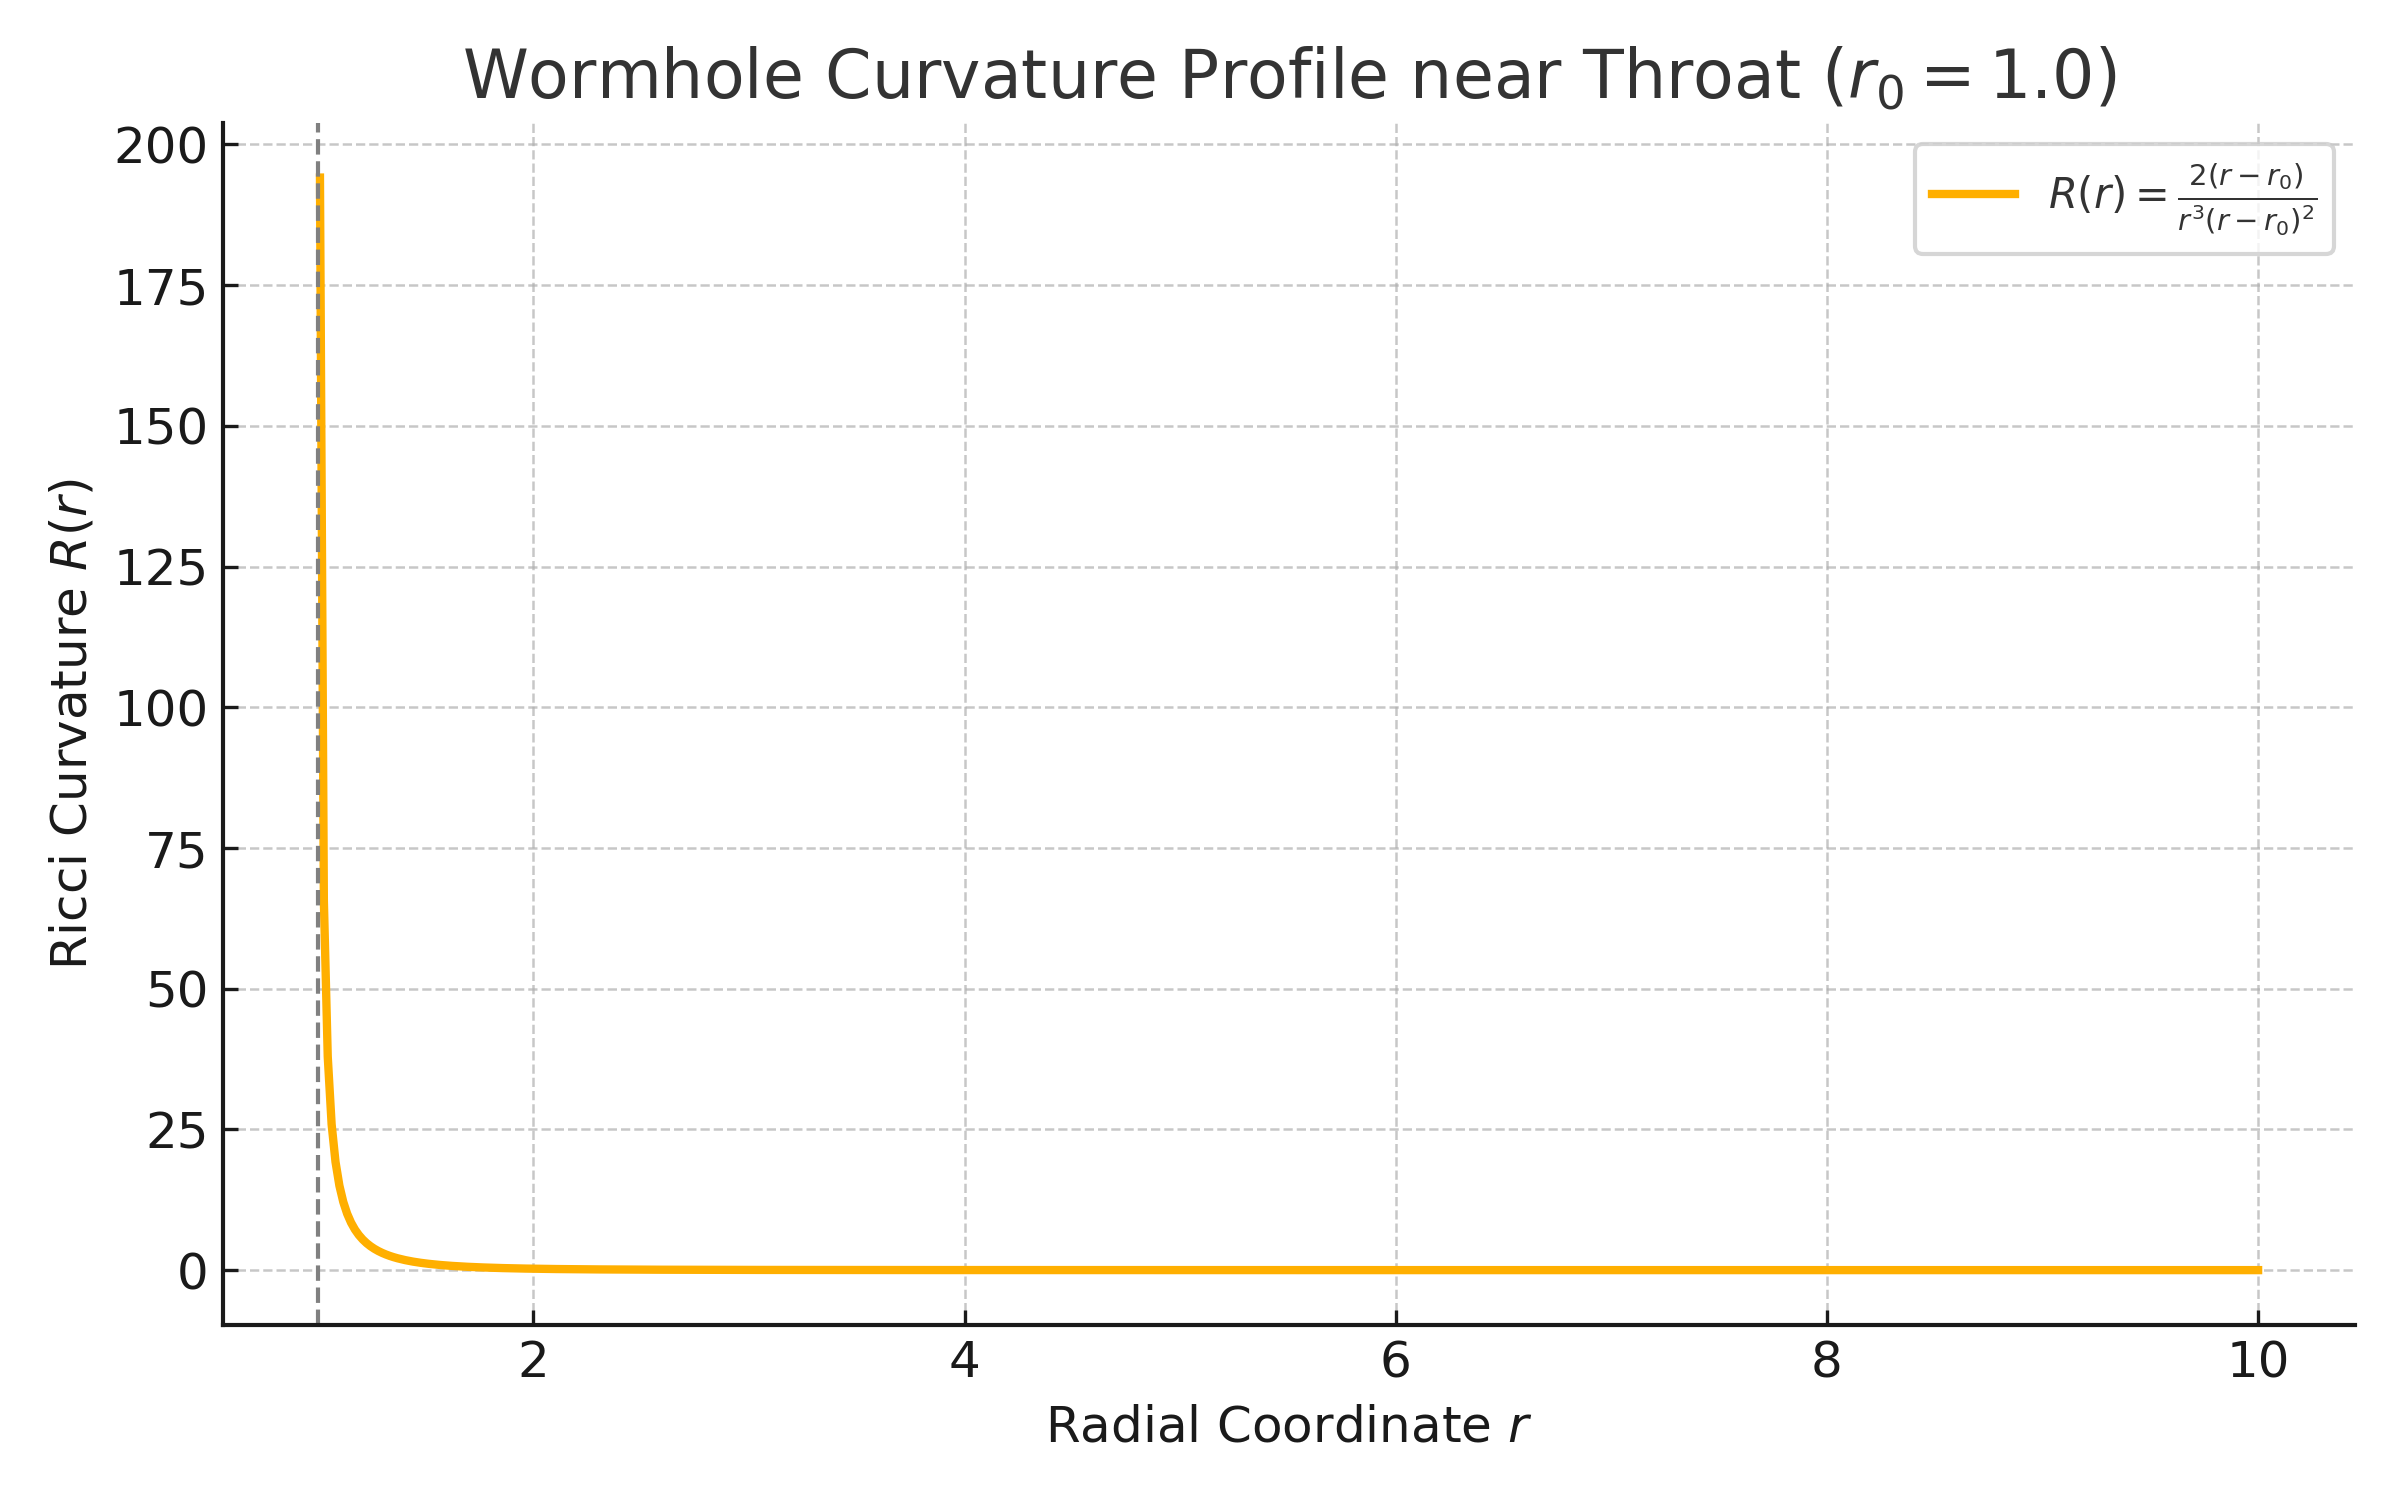
\includegraphics[width=0.85\textwidth]{wormhole_curvature_profile.png}
\caption{Simulated Ricci curvature profile $R(r)$ derived from a Morris--Thorne wormhole metric. As the radial coordinate $r$ approaches the throat $r_0 = 1.0$, curvature increases sharply due to divergence in the redshift function. This profile is used within the WMEV layer to detect geometric instabilities and enforce topological constraints on AI-generated metric embeddings.}
\end{figure}

\section*{Validator Logic (Python)}

\begin{verbatim}
def validate_wormhole_metric(R_profile, r0=1.0, threshold=1e3):
    for r, R in R_profile:
        if abs(r - r0) < 0.1 and abs(R) > threshold:
            return "FAIL: Curvature too high at throat"
    return "PASS: Curvature within acceptable bounds"
\end{verbatim}

\end{document}
